%!TEX root = ../thesis.tex
%*******************************************************************************
%*********************************** Fourth Chapter ****************************
%*******************************************************************************

\chapter{Discussion} %Title of the First Chapter

\ifpdf
    \graphicspath{{Chapter4/Figs/Raster/}{Chapter4/Figs/PDF/}{Chapter4/Figs/}}
\else
    \graphicspath{{Chapter4/Figs/Vector/}{Chapter4/Figs/}}
\fi

The modeling done here offers several perspectives to study the mechanics of sheet shape and inversion in \textit{Choanoeca}. 
We see that the discrete, lattice structure of the sheet makes the sheet's intrinsic curvature possible, and the sheet's curvature emerges in response to the lattice structure.
The presence of topological defects gives a tight ring of cells at the sheet boundary, which presents an energetic challenge during inversion.
The models that I built make it clear that stretching plays a major role in the dynamics of sheet inversion, and they distill the essential mechanics of \textit{C. flexa} colony shape to only two parameters.
This discrete model of sheet inversion supports the hypothesis that \textit{C. flexa} inverts using an instantaneous active change of collar microvillus preferred shape.

%********************************** %First Section  **************************************
\section{\textit{C. flexa} geometry} 

% what does this work achieve
\textit{Choanoeca} differs from its relatives in that it lacks an extracellular matrix, which is responsible for producing disks, cups, or branched trees with flagella splayed out in other species' colonies \citep{larson2020}. 
Despite lacking an ECM, these colonies are able to achieve large-scale geometric changes that are believed to faciliate function \citep{brunet2019}.
In this work, I show that a simple model which distills collar filament mechanics into a few descriptive angles $\phi, \psi$ and filament lengths is sufficient to capture the curvature of whole sheets and their inversions following a rapid stimulus, here captured by an instantaneous change in preferred angles $\phi_0$ and $\psi_0$.
While we can develop increasingly complex models by introducing collar filament bending, tension and stress at the collar filaments' bases, or the effects of the contractile ring, I demonstrate here that a coarse description of individual cells is sufficient to explain the behavior that we observe in colonies. 
Compare this with \textit{Volvox}, which uses connections and communication between cells to control its inversion. 
One might imagine that the complexity of a molecular pathway for a single cell to exhibit phototaxis or regulate feeding/swimming efficiency could easily exceed that of the ring contraction as currently understood in \textit{C. flexa} \citep{brunet2019}. 
\mynote{cite Volvox inversion papers, cite papers on phototaxis or swimming signalling pathways}

% why have a curved sheet?
While the modelling in this work captures the mechanics underlying sheet curvature, it does not identify environmental pressures that may have selected for the morphology exhibited by \textit{Choanoeca} colonies.
The small curvature in \textit{C. flexa} colonies permit them to drive strong flows by aligning their apicobasal axes close to parallel while simultaneously producing two stable shape equilibria.
This contrasts with the rosette colonies of \textit{S. rosetta}, which are known to have morphology inefficient for driving feeding flows \citep{kirkegaard2016}.
\textit{C. flexa} may also be driven to form the observed monolayers of cells because this morphology allows cells more flow of their own for feeding.
Nevertheless, there may be a myriad of other reasons that these species have evolved to have their current morphologies, especially external influences from the ecosystems they inhabit.

% why does choanoeca align as it does
\textit{Choanoeca} is remarkable in the common orientation of all cells in its colonies, which is made possible by its colonies' connections via collar filaments rather than an extracellular matrix \citep{leadbeater1983}. 
It is clear that the collar filaments are essential to the sheet orientation, and that they are the means by which sheets achieve variable curvature.
My work here reduces the complexities of these filaments significantly by representing their bending energies with simple terms based on the angles they make and their end-to-end distances.
Moreover, my discrete model treats the line of filament interactions between two neighbouring cells as a line of many infinitesimal filaments.
A more complete model would explore the details of filament mechanics between cells.
Doubtless, further work on the detailed mechanics contributing to sheet geometry must be guided by experiments.
In particular, it is currently unclear how collar filaments adhere to those of other cells in a seemingly selective way (\cref{subfig:contact1,subfig:contact2}).

\section{Discrete cell sheet topology}

% what did I find about lattice topology?
The discrete model of \textit{C. flexa} demonstrates that deviations from a hexagonally packed sheet at as few as one cell are sufficient to induce substantial bending.
This result is consistent with that described in \citet{seung1988} for planar lattices, albeit through a different mechanism where stretching and bending are closely related.
Indeed, topological defects induce buckling and non-local inability to satisfy equilibrium conditions, yet these defects are also vital to achieving large-scale sheet curvature.
The model I develop in \cref{ch:3} supports the idea that, loosely, defects in the small-scale lattice topology induce curvature in the large-scale sheet geometry.
While not previously explored, we should expect to find a small but non-negligible fraction of cells in \textit{Choanoeca} colonies to have an irregular number of neighbours.
Further imaging as in \cref{subfig:contact1},\ref{subfig:contact2} to quantify the statistics of the numbers of neighbours in colonies would be valuable.

% what do we actually observe and how does it line up with the model used here?
\citet{leadbeater1983} describes that in \textit{C. perplexa} colonies, each cell is typically adjacent to six others. 
Given the strong \textit{Choanoeca} sheet curvatures and known association between Gaussian curvature and topological defects in lattice structure (\cref{subsec:cts}) \citep{sachdev1984,seung1988}, it is reasonable to expect that many cells have more or fewer than six neighbors.
Even in a small section of the colony \cref{subfig:contact1}, several defects may be readily identified.

% How reasonable was this model?
Physical reasoning suggests that interfaces between cells would be equidistant from the cell bodies, since each cell is assumed to be identical and the forces must balance at equilibrium. 
Imaging supports this idea (\cref{fig:cflexa}), though any imaging requiring fixation may affect the collar stiffness or preferred curvature.
That the collar microvilli at the boundaries form an arc around the apicobasal axis suggests that they freely take angle $\phi_0$ at the base and do not contribute meaningfully to the energy (\cref{subfig:contact2}). 
This validates the treatment of boundary collar vertices used in the discrete model.

\section{Extensions}

% studying what prevents inversion
Both the continuous and discrete models developed make clear that azimuthal stretching in curved sheets is critical in \textit{C. flexa} inversion, especially by introducing an energetic barrier.
With even relatively large-area sheets observed inverting readily in culture (collar diameter relative to sheet major-axis diameter as low as $\sim20\%$), collar-collar interfaces must either be able to substantially stretch or connections must break.

% more detailed flow
The simple, continuous one-dimensional model of \cref{sec:c_1d} had two clear limitations discussed there: the lack of chain elongation or shortening and the assumption of linear, isotropic drag.
The results discussed in this work support the hypothesis that the former is largely responsible for \textit{Choanoeca} colony shape.
However, the extent to which flow affects sheet shape is unclear, both in experimental results \citep{brunet2019} as well as the larger theoretical work this thesis contributes to.
Linear, local isotropic drag would suggest a chain of cells falling through the fluid has the same shape as it falls, yet intuitively we expect the ends of the chain to lag behind its centre.
I expect that the effect would be less pronounced in a two-dimensional sheet since azimuthal stretching and compression generally appear to restrict sheet shape (\cref{fig:extra}), though there are nevertheless many questions to explore relating flow and geometry.
Consequently, we should be careful to draw conclusions from details in the dynamics of the models presented here, including \cref{fig:shapes} and \cref{fig:dynamics}.
Since the shape changes in the discrete model are slow relative to the timescale defined by system size and fluid properties, it is compelling to at least treat sheet boundaries rolling over as a consequence of topological constraints.
Our understanding of flow's impact on colony shape would be improved greatly by experiments placing colonies near surfaces or in external flows and observing any changes in shape.

% describing colony growth and resulting lattice topology
A model for \textit{Choanoeca} colony growth may help understand the origins and distributions of topological defects in the lattice structure. 
Given the possible division strategy of these cells (\cref{fig:division}) and the idea that other choanoflagellate colony cells divide without synchronisation \citep{larson2020}, we might build a model by spontaneously splitting cells into pairs of adjacent daughter cells.
The goal of a colony growth model is two-fold.
First, a model for colony growth may explain the origin of topological defects in \textit{C. flexa} colonies.
We would obtain graph topological statistics that are comparable to experiments to determine if this method of colony growth is accurate or if another method produces the observed topological defects.
Second, such a model may cause the cup-like sheets observed, rather than sheets with other complex geometries.
Moreover, the distribution of defects over the sheet may produce non-icosahedral or -spherical equilibrium geometries, as large \textit{Choanoeca} sheets tend to be ellipsoidal rather than spherical \citep{leadbeater1983,brunet2019}.
It remains to be resolved how colonies form without buckling at sheet boundary: uniform, isotropic cell division would give proportionally scaling area and boundary length, but preferred sheet curvature would cause buckling with too large of a boundary.
We can consider this as a conflict between preferred sheet curvature with bending based on $\sin (\psi_0 - \phi_0)$ and preferred cell space based on $\ell_0 \sin \phi_0$ (\cref{eq:h0}).
Experimental observations of colonies as they grow and divide would validate a model for growth, as well as provide some insight into the formation, coordination, and persistence of collar-collar connections.

% alternative colony growth theorising
An alternative theory for \textit{Choanoeca} colony growth is via aggregation \citep{grosberg2007}, though choanoflagellate colonies have only been observed to form by clonal division \citep{fairclough2010,alegado2012,woznica2016}.
Sequential cell adhesion at the boundary would resolve buckling at the edges due to uniform, isotropic growth.
Moreover, aggregation resolves the issue that there are a discrete number of microvilli at cell-cell interfaces.
Hence, the interfaces cannot be divided between daughter cells indefinitely.
Recent evidence from \textit{S. rosetta} points that several processes involved in maintaining the colony ECM are involved in preventing spurious aggregation \citep{wetzel2018}, indicating that aggregation is specifically disfavored in other choanoflagellates.
Colony formation by aggregation is unprecendented in our understanding of choanoflagellates, and of course comes with the organisational challenge of producing a single consistent orientation over the entire sheet.

% changing lattice topology to induce inversion
While the structures used in this work had discrete symmetry around an axis, \textit{C. flexa} sheets observed experimentally may have substantial irregularities both in the bulk and at the boundary. 
Several images in \citet{brunet2019} show uneven sheet boundaries, resembling crenellations of a castle wall (\cref{fig:edges}).
As suggested in \cref{subsec:dynamics}, a sheet with excessively restrictive lattice topology may be able to achieve inversion by a temporary change in its cell-cell connections, especially by tearing or forming holes in the sheet.
Continued experimental work should look for disconnections between adjacent cells between inversion.
An extreme example of inversion through topological change is performed by \textit{Volvox} embryos, which invert by creating a hole in their sphere and pass the entire sheet through the hole \citep{hohn2015}.
Type-A \textit{Volvox} inversion forms this hole by making four lips and peels them back to begin inversion at the boundary, similar to how inversion proceeds in \cref{fig:dynamics} \citep{viamontes1977}.
Even besides boundary ruggedness, asymmetry in the sheet may promote the initiation of inversion at one region of the boundary while it is not yet possible elsewhere.

% how do colonies break apart?
\citet{leadbeater1983} described that large \textit{C. perplexa} sheets may take irregular shapes such as ribbons. 
Either as a consequence of tearing during inversion or itself causing tearing during inversion, such unusual geometries may be involved in colony division.
If colonies tear, we would not expect them to fully separate since a single connection at the boundary of either colony fragment would not hinder inversion. 
Consequently, it is possible that the weight of colony fragments themselves in the flagella-in state (with resulting incompatible drag tensors) or the strong collective flows driven by separate colony fragments in the flagella-out state are responsible for separating colony fragments.
If entirely physically facilitated, colony division is likely to substantially involve both cell-cell connection lattice structure and flows.

% assuming all cells are the same
An underlying assumption throughout this work is that \textit{Choanoeca} colonies consist entirely of identical cells, both in genetics and morphology.
Recent findings in \textit{S. rosetta} suggest that choanoflagellates are capable of spatial differentiation within colonies \citep{laundon2019,naumann2019}.
Different properties throughout the cell-cell connection network, especially different preferred collar shapes due to cell body morphology or filament mechanics, substantially affect inversion dynamics.
Most substantial would be if some adjacent cells do not form adhesive contact at all, in contrast to our current interpretation of \textit{Choanoeca} colony imaging \citep{brunet2019}.

\begin{figure}
	\centering
	\begin{subfigure}[b]{0.46\textwidth}
		\centering
		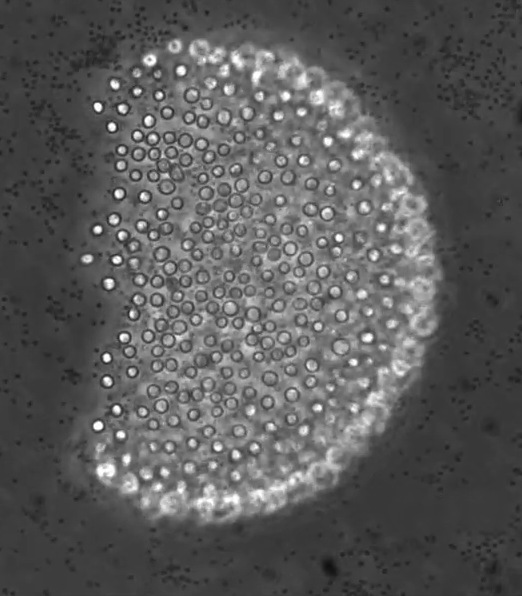
\includegraphics[height=\textwidth,angle=90]{edges1.png}
		\caption{}
		\label{subfig:edges1}
	\end{subfigure}
	\begin{subfigure}[b]{0.49\textwidth}
		\centering
		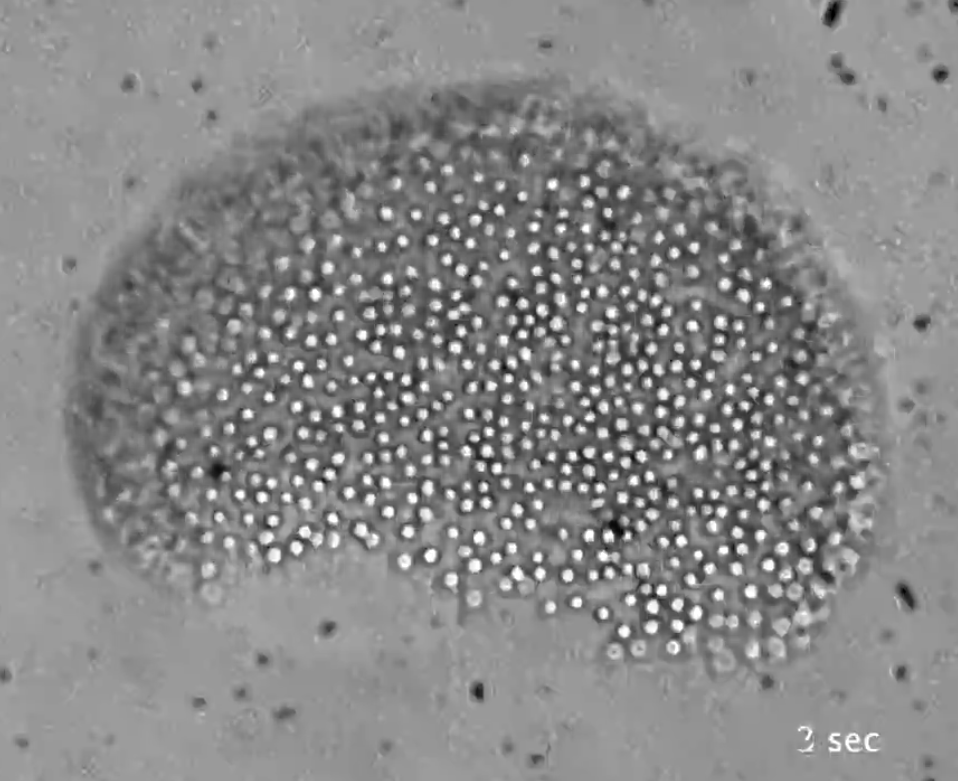
\includegraphics[width=\textwidth]{edges2.png}
		\caption{}
		\label{subfig:edges2}
	\end{subfigure}
	\caption[\textit{C. flexa} sheets with ragged boundaries]{\textit{C. flexa} sheets with ragged boundaries. From \citet{brunet2019}. Reprinted with permission from AAAS.}
	\label{fig:edges}
\end{figure}

\section{Multicellularity and \textit{C. flexa}}

% \textit{C. flexa} contrasts with volvocine algae because it does not connect cells via cytoplasmic bridges, which is a substantial difference between the two models. 
% It is not completely clear that \textit{C. flexa} sheets form with a temporary incomplete cytokinesis stage as in the algae \citep{green1981,herron2015}.

Ultimately, multicellularity in \textit{Chonoaeca} appears to be the result of a tradeoff between a decrease in the flow efficiency of individual choanoflagellate cells and the ability of the colony to invert. 
Inversion is highly dependent on the sheet structure and its lattice, which may itself change to facilitate inversion and potentially colony divison. 
A more complete experimental characterisation of \textit{Choanoeca} colonies would further inform the models developed here and clear up the connection between lattice topology, inversion, colony formation, and colony division.
Nevertheless, the multicellular mechanics of \textit{C. flexa} are crucial to its inversion and the behavior that inversion make possible.
